\clearpage
\subsection{LM-band long-slit spectroscopy recipes}
\label{ssec:recipes_lss_lm}

A draft of the reduction cascade is shown in
Figs.~\ref{Fig:LMLssAssomap1} and \ref{Fig:LMLssAssomap2}. The first part aims to update the static calibration database, in particular the creation of the gain map (\REC{metis_det_lingain}) and the determination of the \ac{ADC} slitlosses (\REC{metis_lm_adc_slitloss}). They are executed only when an update is required, e.g. after a major instrument intervention or on yearly basis. The second part comprises the basic calibrations, e.g. the dark correction and the spectroscopic flatfielding via \ac{RSRF}, followed by the third part, the main calibration steps, incorporating the determination of the first guess wavelength solution by means of the laser sources in the \ac{WCU} and the determination of the response curve for the flux calibration. Subsequently, the main reduction is conducted, which applies the previously created master calibration files to the science frames. Both, the standard star and the science observations are wavelength calibrated with the help of the atmospheric lines visible in the respective spectra. Therefore the main step of the wavelength calibration is carried out in the recipes \REC{metis_lm_lss_std} and \REC{metis_lm_lss_sci}. Finally, the telluric absorption correction is applied using the modelling approach with \texttt{molecfit}. Optionally, the telluric correction can be done with a telluric standard star.\\
Note that the list of \ac{QC} parameters in the recipe descriptions will be extended whenever necessary.\\

\subsubsection{\REC*{metis_det_lingain} and \REC*{metis_det_dark}: Linearity/Gain}
These recipes aim for detector-specific calibrations and are therefore the same as in the imaging pipeline. Common detector calibrations are described in Section~\ref{Sec:detector_calibration}.

%------------------------------------------------------------------------------------------------------------------
\subsubsection{\REC*{metis_lm_adc_slitloss}: Slit loss determination}
The recipe \REC{metis_lm_adc_slitloss} aims to determine the slit losses induced by the fixed \ac{ADC} positions as function of the object position across the slit. The recipe aims to create a table with slitlosses (\STATCALIB{LM_ADC_SLITLOSS}), which is added to the static database and used in the recipes \REC{metis_lm_lss_std}. This recipe is to be carried out only when an update of the database is needed. The algorithm and the workflow of the recipe to determine the slit-losses is given in Section~\ref{sssec:adc_slitlosses}, more information can be found in Section "Calibration of slit-losses" in the Calibration Plan~\cite{METIS-calibration_plan}. 


%------------------------------------------------------------------------------------------------------------------
\subsubsection{\REC*{metis_lm_lss_rsrf}:  Flatfielding}\label{rec:metis_lm_lss_rsrf}
The recipe \REC{metis_lm_lss_rsrf} aims to create a spectroscopic master flatfield for determining the pixel-to-pixel sensitivity and to enable the order location algorithm (\REC{metis_lm_lss_trace}).
\begin{figure}[ht]
  \centering
  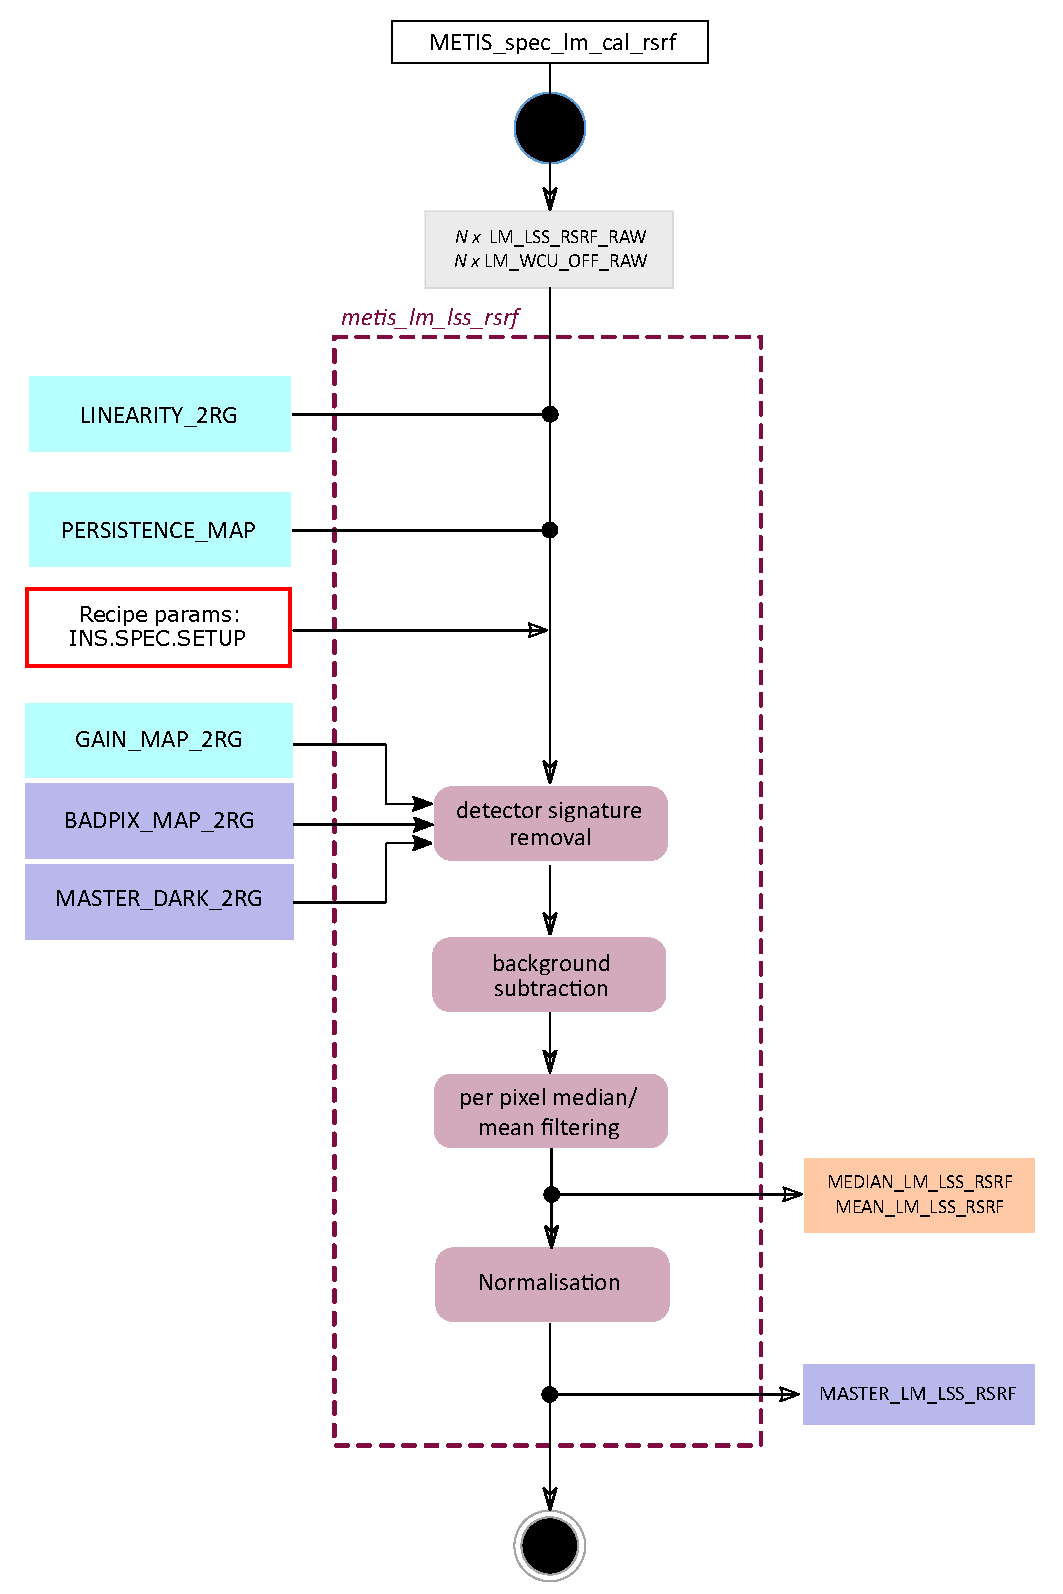
\includegraphics[width=0.5\textheight]{figures/metis_lm_lss_rsrf_v0.84.pdf}
    \notgenerated{flowchart: hand-drawn; the recipe declares no steps}
  \caption[Recipe: \REC*{metis_lm_lss_rsrf}]{\REC*{metis_lm_lss_rsrf} --
    Recipe workflow to create the spectroscopic flatfield by means of the \ac{RSRF}.}
  \label{Fig:rec_lm_lss_rsrf}
\end{figure}

\begin{recipedef}
  Name:                & \REC{metis_lm_lss_rsrf} \\
  Purpose:             & Create spectroscopic relative spectral response function (RSRF) for the 2RG detector \\
%  Requirements:        & \REQ{METIS-XXXX} \\
%  Type:                & Calibration | Science | Technical \\
%  Templates:           & \TPL{...} \\
  Primary input:       & \RAW{LM_LSS_RSRF_RAW} (N$\times$) \\
                       & \RAW{LM_WCU_OFF_RAW} (N$\times$) \\
  Secondary inputs:    & \PROD{BADPIX_MAP_2RG} (optional) \\
                       & \hyperref[dataitem:gain_map_det]{\STATCALIB*{GAIN_MAP_2RG}} \\
                       & \hyperref[dataitem:linearity_det]{\PROD*{LINEARITY_2RG}} \\
                       & \PROD{MASTER_DARK_2RG} \\
                       & \EXTCALIB{PERSISTENCE_MAP} (optional) \\
  Matched keywords:    & \FITS{DET.DIT} \\
                       & \FITS{DET.NDIT} \\
                       & \FITS{DRS.SLIT} \\
  Parameters:          & \CODE{metis_lm_lss_rsrf.stacking.method}: string\newline Name of the method used to combine the input images (\texttt{average}, \underline{\texttt{median}}) \\
  Algorithm:           & Fancy algorithm description follows ***TBD*** \\
  Output data:         & \PROD{MASTER_LM_LSS_RSRF} \\
                       & \PROD{MEAN_LM_LSS_RSRF} \\
                       & \PROD{MEDIAN_LM_LSS_RSRF} \\
%  Expected accuracies: & \\
  QC1 parameters:      & \QC{QC LM LSS RSRF INTORDR LEVEL} \\
                       & \QC{QC LM LSS RSRF MEAN LEVEL} \\
                       & \QC{QC LM LSS RSRF MEDIAN LEVEL} \\
                       & \QC{QC LM LSS RSRF NORM SNR} \\
                       & \QC{QC LM LSS RSRF NORM STDEV} \\
\end{recipedef}


\clearpage

%------------------------------------------------------------------------------------------------------------------
\subsubsection{\REC*{metis_lm_lss_trace}:  Order detection}\label{rec:metis_lm_lss_trace}
The recipe \REC{metis_lm_lss_trace} aims at detecting the order and a polynomial fitting of the order location (see~\cite{pis02} and~\cite{pis21} for details on the algorithms). The detection and polynomial fitting is based on flatfield frames taken through a pinhole mask, which leads to individual pinhole traces along the entire dispersion direction.

\begin{figure}[ht]
  \centering
  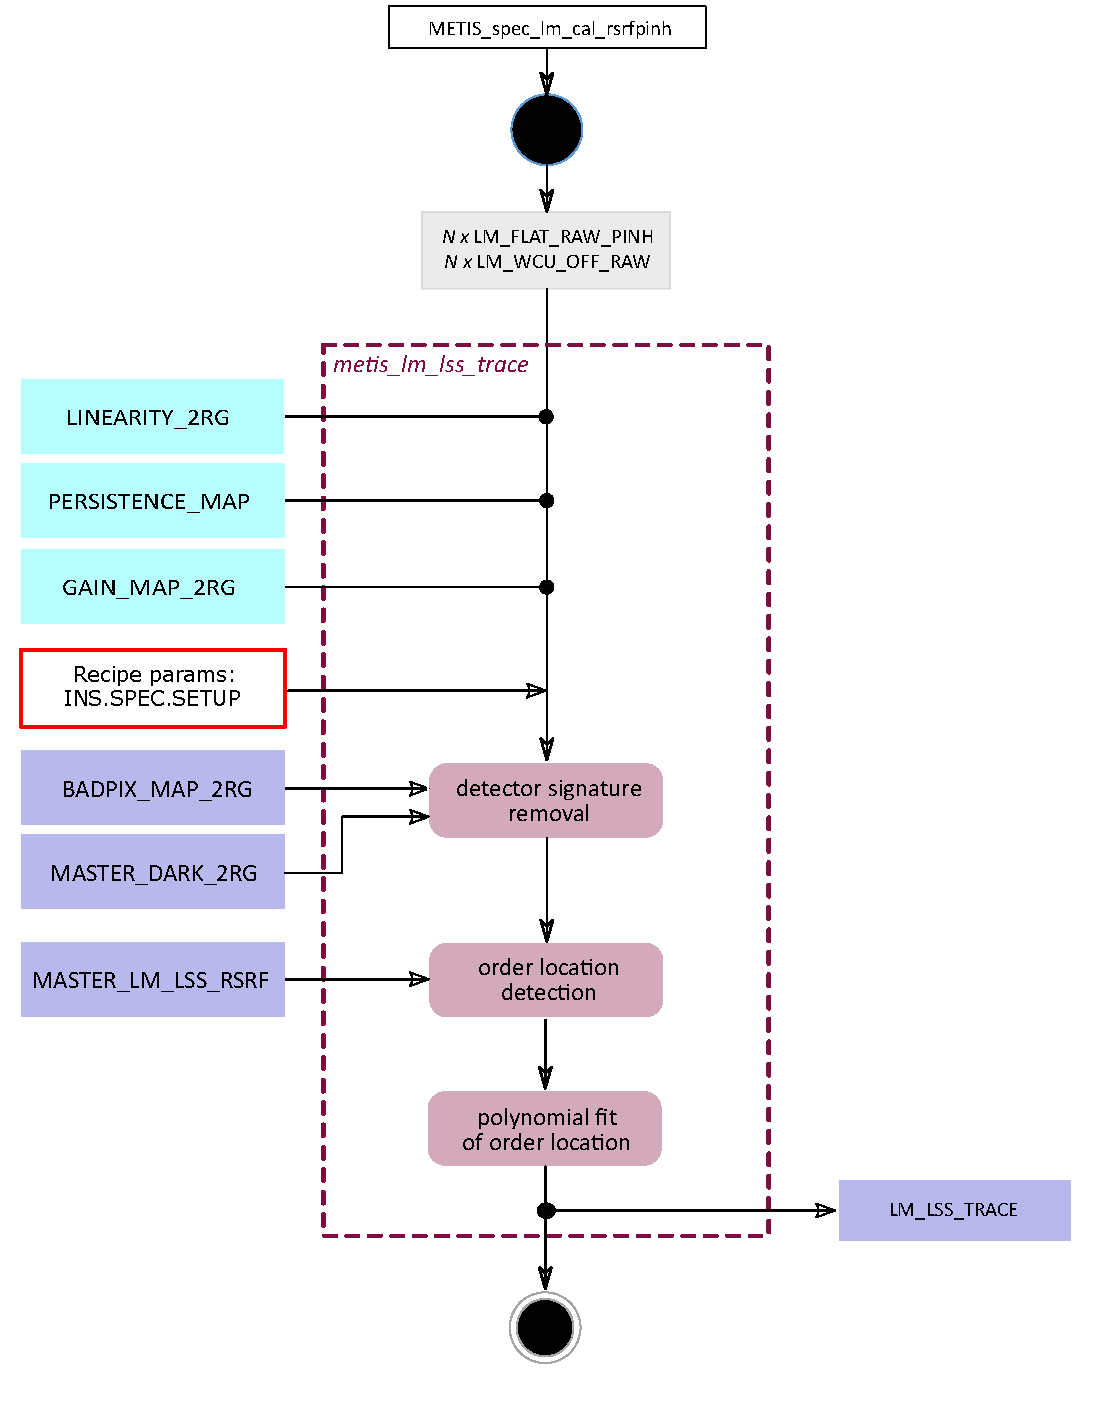
\includegraphics[width=0.5\textheight]{figures/metis_lm_lss_trace_v0.84.pdf}
    \notgenerated{flowchart: hand-drawn; the recipe declares no steps}
  \caption[Recipe: \REC*{metis_lm_lss_trace}]{\REC*{metis_lm_lss_trace} --
    Detection and polynomial fitting of the order location.}
  \label{Fig:rec_lm_lss_wtrace}
\end{figure}

\begin{recipedef}
  Name:                & \REC{metis_lm_lss_trace} \\
  Purpose:             & Detection of LM order location on the 2RG detector \\
%  Requirements:        & \REQ{METIS-XXXX} \\
%  Type:                & Calibration | Science | Technical \\
%  Templates:           & \TPL{...} \\
  Primary input:       & \RAW{LM_LSS_RSRF_PINH_RAW} (1--N) \\
                       & \RAW{LM_WCU_OFF_RAW} (1--N) \\
  Secondary inputs:    & \PROD{BADPIX_MAP_2RG} (optional) \\
                       & \hyperref[dataitem:gain_map_det]{\STATCALIB*{GAIN_MAP_2RG}} \\
                       & \hyperref[dataitem:linearity_det]{\PROD*{LINEARITY_2RG}} \\
                       & \PROD{MASTER_DARK_2RG} \\
                       & \PROD{MASTER_LM_LSS_RSRF} \\
                       & \EXTCALIB{PERSISTENCE_MAP} (optional) \\
  Matched keywords:    & \FITS{DET.DIT} \\
                       & \FITS{DET.NDIT} \\
                       & \FITS{DRS.SLIT} \\
  Parameters:          & \CODE{metis_lm_lss_trace.parameter1}\newline Description of parameter 1 (\texttt{value2}, \texttt{value1}), default \texttt{value1} \\
  Algorithm:           & Fancy algorithm description follows ***TBD*** \\
  Output data:         & \PROD{LM_LSS_TRACE} \\
%  Expected accuracies: & \\
  QC1 parameters:      & \QC{QC LM LSS TRACE INTORDR LEVEL} \\
                       & \QC{QC LM LSS TRACE LCOEFForder} \\
                       & \QC{QC LM LSS TRACE LPOLYDEG} \\
                       & \QC{QC LM LSS TRACE RCOEFForder} \\
                       & \QC{QC LM LSS TRACE RPOLYDEG} \\
\end{recipedef}



\clearpage
%------------------------------------------------------------------------------------------------------------------
\subsubsection{\REC*{metis_lm_lss_wave}:  Wavelength calibration}\label{rec:metis_lm_lss_wave}
This recipe aims at determining the first guess of the wavelength calibration on basis of the \ac{WCU} laser sources (c.f. \cite{METIS-calibration_plan}). Therefore the first steps are the removal of the detector signature of the \RAW*{LM_WAVE_RAW} frames by applying the master calibration files derived in the previous steps, following by the background subtraction (if needed) and the application of the RSRF. The distortion of the lines (i.e. possible tilt, curvature,...) and the wavelength solution is determined by the algorithm developed by Piskunov et al. (\cite{pis02}, \cite{pis21}). The reference frame is defined by the laser line catalogue (\STATCALIB{LASER_TAB}).\\
This is in compliance with \REQ{METIS-6074}.\\
\textit{Remark:}  For the N-band there will be laser sources only at \ac{AIT} available, from which we derive the first guess solution in the same way. Although this solution will eventually be put into the static calibration database, we need a recipe to process the N-band data. This will be done with this recipe.

\begin{figure}[ht]
  \centering
  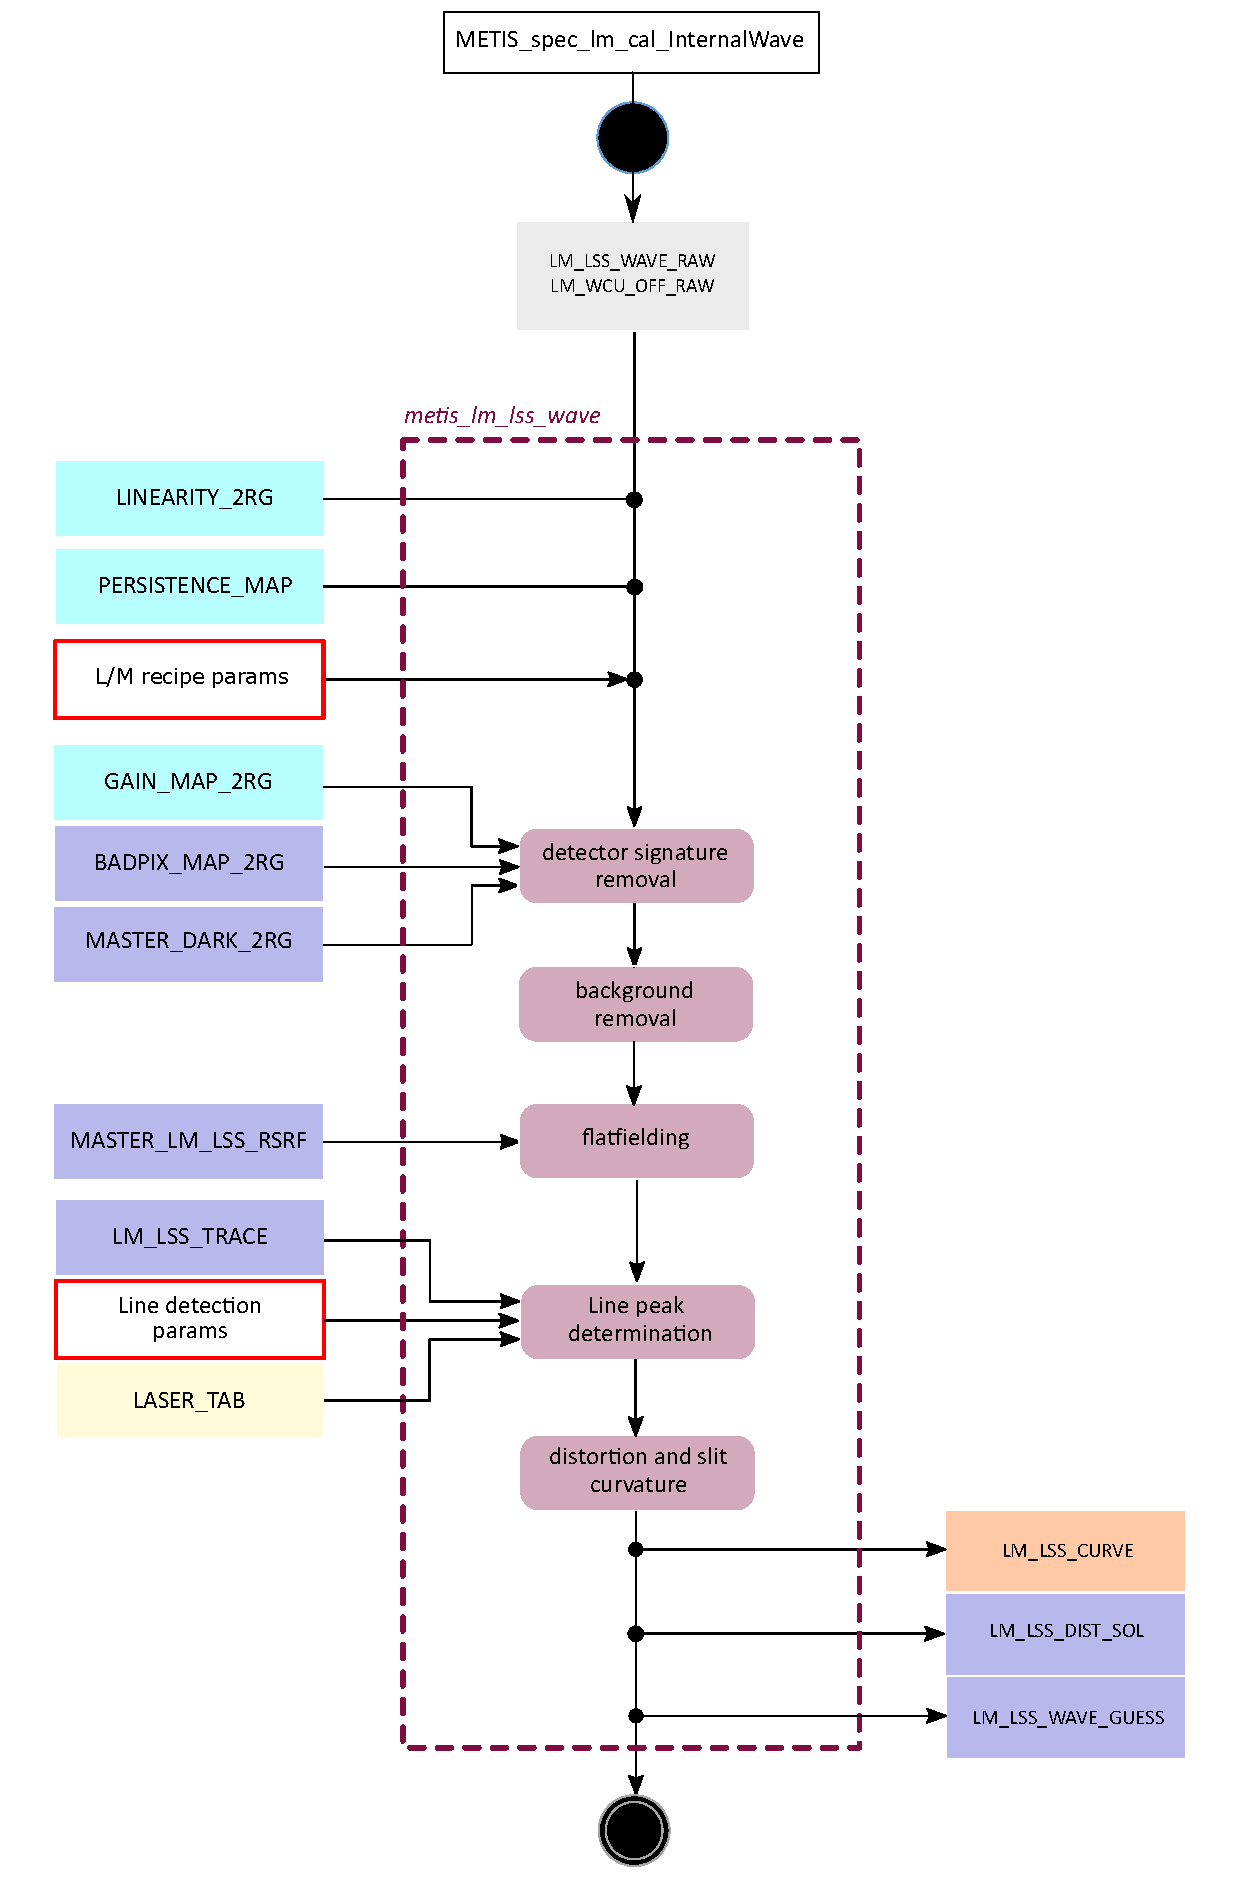
\includegraphics[width=0.5\textheight]{figures/metis_lm_lss_wave_v0.84.pdf}
    \notgenerated{flowchart: hand-drawn; the recipe declares no steps}
  \caption[Recipe: \REC*{metis_lm_lss_wave}]{\REC*{metis_lm_lss_wave} --
    Creation of the LM LSS master wavelength correction.}
  \label{Fig:rec_lm_lss_trace}
\end{figure}
\clearpage

\begin{recipedef}
  Name:                & \REC{metis_lm_lss_wave} \\
  Purpose:             & First guess of the wavelength solution based on WCU laser reference \\
%  Requirements:        & \REQ{METIS-XXXX} \\
%  Type:                & Calibration | Science | Technical \\
%  Templates:           & \TPL{...} \\
  Primary input:       & \RAW{LM_LSS_WAVE_RAW} (N$\times$) \\
                       & \RAW{LM_WCU_OFF_RAW} (N$\times$) \\
  Secondary inputs:    & \PROD{BADPIX_MAP_2RG} \\
                       & \hyperref[dataitem:gain_map_det]{\STATCALIB*{GAIN_MAP_2RG}} \\
                       & \EXTCALIB{LASER_TAB} \\
                       & \hyperref[dataitem:linearity_det]{\PROD*{LINEARITY_2RG}} \\
                       & \PROD{LM_LSS_TRACE} \\
                       & \PROD{MASTER_DARK_2RG} \\
                       & \PROD{MASTER_LM_LSS_RSRF} \\
                       & \EXTCALIB{PERSISTENCE_MAP} (optional) \\
  Matched keywords:    & \FITS{DET.DIT} \\
                       & \FITS{DET.NDIT} \\
                       & \FITS{DRS.SLIT} \\
  Parameters:          & \CODE{metis_lm_lss_wave.parameter1}: string\newline Description of parameter 1 (\texttt{value2}, \underline{\texttt{value1}}) \\
  Algorithm:           & Fancy algorithm description follows ***TBD*** \\
  Output data:         & \PROD{LM_LSS_CURVE} \\
                       & \PROD{LM_LSS_DIST_SOL} \\
                       & \PROD{LM_LSS_WAVE_GUESS} \\
%  Expected accuracies: & \\
  QC1 parameters:      & \QC{QC LM LSS WAVE COEFFi} \\
                       & \QC{QC LM LSS WAVE INTORDR LEVEL} \\
                       & \QC{QC LM LSS WAVE LINEFWHMAVG} \\
                       & \QC{QC LM LSS WAVE NLINES} \\
                       & \QC{QC LM LSS WAVE POLYDEG} \\
\end{recipedef}



\clearpage
%------------------------------------------------------------------------------------------------------------------
\subsubsection{\REC*{metis_lm_lss_std}:  Standard star processing}\label{rec:metis_lm_lss_std}
This recipe aims at processing standard stars used for the absolute flux calibration and (optionally) for the telluric feature removal: As first step the detector master calibration files derived previously are applied followed by the background subtraction, if needed the distortion correction (\PROD{LM_LSS_DIST_SOL}), and
the wavelength calibration by means of the first guess solution (\PROD{LM_LSS_WAVE_GUESS}) and the telluric sky lines (c.f. Sect.\,8.5 in~\cite{DRLS}). Then the recipe removes sky background, extracts the standard star spectrum object and collapses the 2D to 1D spectra. In case the \ac{STD} is used only for the flux calibration, a telluric correction is required to better compare the corresponding model spectrum. This is done by means of the standard star observations itself or (optionally) with a synthetic transmission curve (either a standard curve derived by the ESO Skycalc Tool\footnote{\url{https://www.eso.org/observing/etc/bin/gen/form?INS.MODE=swspectr+INS.NAME=SKYCALC}}, a standard curve (\STATCALIB{LM_SYNTH_TRANS}) or \texttt{molecfit}. It is on the user's decision whether the standard star is used for the absolute flux calibration only, or also used for the telluric correction of the science target. The response function is then calculated as ratio of the measured 1d-\ac{STD} spectrum and a detailed model containing absolute flux information.

%As one needs to determine the stellar continuum regions, a telluric correction is required to increase these regions. This can be done either by applying a fairly simple telluric correction in an automated way to the standard star spectrum. In case the the user decides to use the standard star also for the telluric correction, a transmission function is derived from that in the "classical" way (cf. Section~\ref{sssec:tecllcorrclassic}), which will be optionally used for the telluric correction also for the science target. This star spectrum can also be optionally used for the wavelength solution and for the flux calibration, if the \ac{TSS} is suited for that. The response curve is obtained by comparing the extracted spectrum with a model and/or another reference spectrum of the standard star. Currently it is foreseen to use the same standard stars as in \ac{CRIRES}/CRIRES+ and \ac{VISIR}. It is under investigation whether more stars are needed.

Please note that the procedure of the \ac{STD} handling changes when the classical method for the telluric correction is chosen. The reason is that in the response function, also the telluric features of the \ac{STD} star have to be present to be able to apply a combination of the telluric absorption removal and the conversion towards physical flux units (cf. Section~\ref{ssec:tellcorr}). In the case of using \texttt{molecfit}, a telluric correction is applied to the \ac{STD} spectrum to better determine the response function and only the response is delivered to the science recipes. In case of the classical approach with a \ac{STD}, the response function will also contain the telluric features of the \ac{STD}, and therefore a telluric correction beforehand is counterproductive.\\

\begin{figure}[ht]
  \centering
  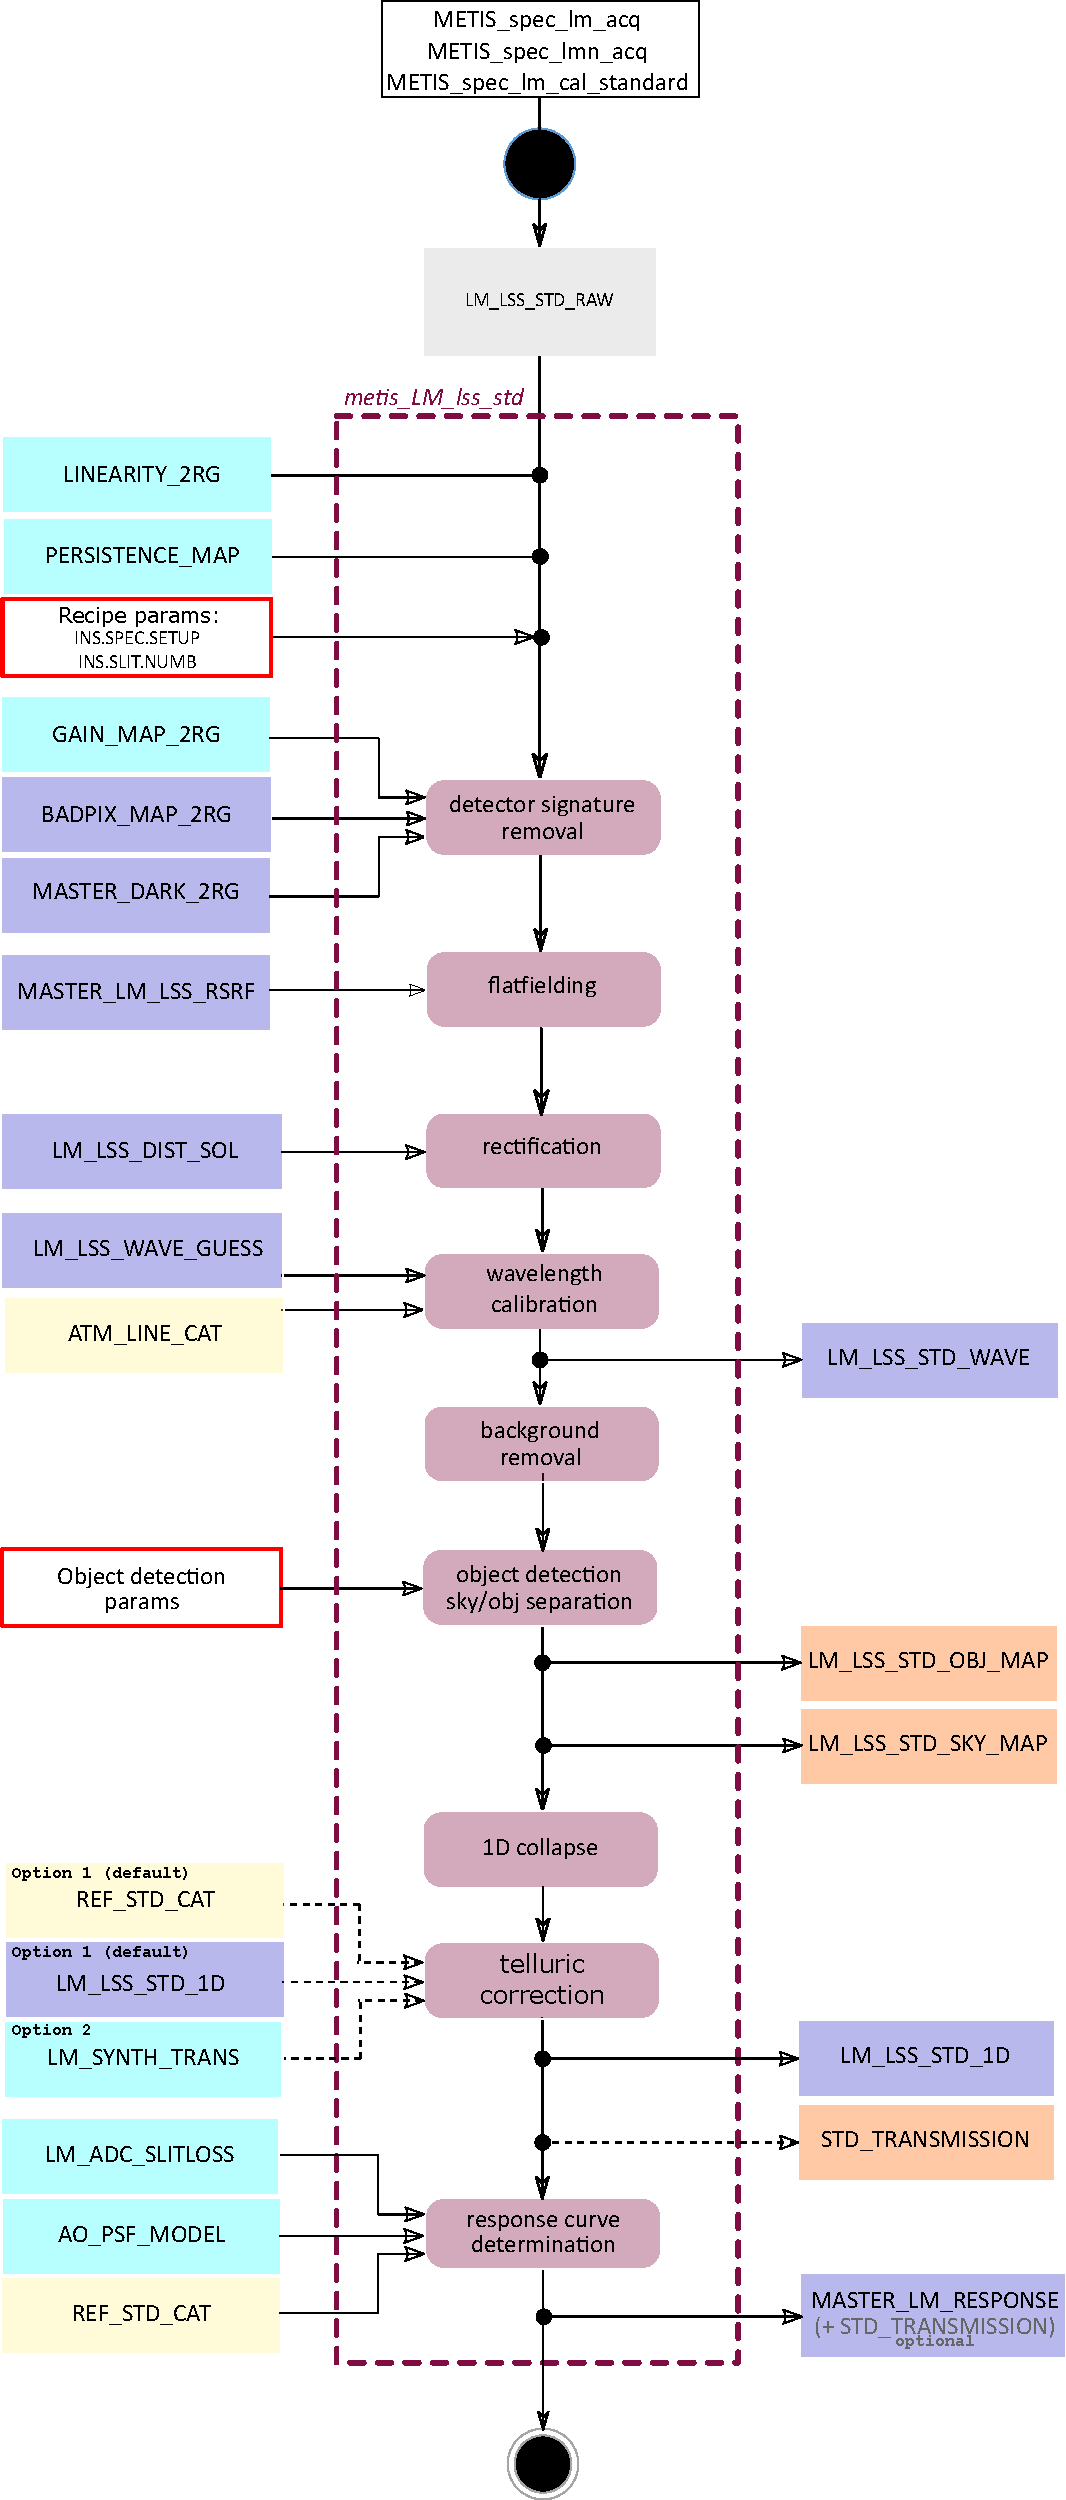
\includegraphics[width=0.4\textheight]{figures/metis_lm_lss_std_v0.83.pdf}
    \notgenerated{flowchart: hand-drawn; the recipe declares no steps}
  \caption[Recipe: \REC*{metis_lm_lss_std}]{\REC*{metis_lm_lss_std} --
    Calibration recipe for processing standard stars for (combined) telluric and  spectro-photometric calibration.}
  \label{Fig:rec_lm_lss_flux1}
\end{figure}
%\begin{figure}[ht]
%  \centering
%  \includegraphics[width=0.6\textheight]{figures/metis_lm_lss_std_v0.8_part_2.pdf}
%  \caption[Recipe: \REC*{metis_lm_lss_std}]{\REC*{metis_lm_lss_std} --
%    Part 2 of the calibration recipe for processing spectrophotometric and telluric standard stars.}
%  \label{Fig:rec_lm_lss_flux2}
%\end{figure}
\clearpage
\begin{recipedef}
  Name:                & \REC{metis_lm_lss_std} \\
  Purpose:             & Reduction of the standard star frames for determining the response function (flux calibration) and/or the transmission (telluric correction) \\
%  Requirements:        & \REQ{METIS-XXXX} \\
%  Type:                & Calibration | Science | Technical \\
%  Templates:           & \TPL{...} \\
  Primary input:       & \RAW{LM_LSS_STD_RAW} (1--N) \\
  Secondary inputs:    & \EXTCALIB{AO_PSF_MODEL} \\
                       & \EXTCALIB{ATM_LINE_CAT} \\
                       & \PROD{BADPIX_MAP_2RG} (optional) \\
                       & \hyperref[dataitem:gain_map_det]{\STATCALIB*{GAIN_MAP_2RG}} \\
                       & \hyperref[dataitem:linearity_det]{\PROD*{LINEARITY_2RG}} \\
                       & \STATCALIB{LM_ADC_SLITLOSS} \\
                       & \PROD{LM_LSS_DIST_SOL} \\
                       & \PROD{LM_LSS_WAVE_GUESS} \\
                       & \STATCALIB{LM_SYNTH_TRANS} \\
                       & \PROD{MASTER_DARK_2RG} \\
                       & \PROD{MASTER_LM_LSS_RSRF} \\
                       & \EXTCALIB{PERSISTENCE_MAP} \\
                       & \STATCALIB{REF_STD_CAT} \\
  Matched keywords:    & \FITS{DET.DIT} \\
                       & \FITS{DET.NDIT} \\
                       & \FITS{DRS.SLIT} \\
  Parameters:          & \CODE{metis_lm_lss_std.parameter1}\newline Description of parameter 1 (\texttt{value2}, \texttt{value1}), default \texttt{value1} \\
  Algorithm:           & Fancy algorithm description follows ***TBD*** \\
  Output data:         & \PROD{LM_LSS_STD_1D} \\
                       & \PROD{LM_LSS_STD_OBJ_MAP} \\
                       & \PROD{LM_LSS_STD_SKY_MAP} \\
                       & \PROD{LM_LSS_STD_WAVE} \\
                       & \PROD{MASTER_LM_RESPONSE} \\
                       & \PROD{STD_TRANSMISSION} \\
%  Expected accuracies: & \\
  QC1 parameters:      & \QC{QC LM LSS STD AVGLEVEL} \\
                       & \QC{QC LM LSS STD BACKGD MEAN} \\
                       & \QC{QC LM LSS STD BACKGD MEDIAN} \\
                       & \QC{QC LM LSS STD BACKGD STDEV} \\
                       & \QC{QC LM LSS STD FWHM} \\
                       & \QC{QC LM LSS STD INTORDR LEVEL} \\
                       & \QC{QC LM LSS STD NOISELEV} \\
                       & \QC{QC LM LSS STD PSFLOSS} \\
                       & \QC{QC LM LSS STD SNR} \\
                       & \QC{QC LM LSS STD WAVECAL DEVMEAN} \\
                       & \QC{QC LM LSS STD WAVECAL FWHM} \\
                       & \QC{QC LM LSS STD WAVECAL NIDENT} \\
                       & \QC{QC LM LSS STD WAVECAL NMATCH} \\
                       & \QC{QC LM LSS STD WAVECAL POLYCOEFFn} \\
                       & \QC{QC LM LSS STD WAVECAL POLYDEG} \\
\end{recipedef}


%------------------------------------------------------------------------------------------------------------------
\clearpage
\subsubsection{\REC*{metis_lm_lss_sci}:  Science reduction}\label{rec:metis_lm_lss_sci}
The science calibration recipe comprises the extraction of the object (i.e. separation of object/sky pixels), removing the sky lines, the application of the response curve previously defined. In case of a point/compact source, the 2D to 1D collapse is also done, otherwise 2D products are delivered. Finally, the spectra are coadded. The recipe also applies an absolute flux calibration (optionally with the telluric correction in one step, cf. Section~\ref{ssec:tellcorr}).
\begin{figure}[ht]
  \centering
  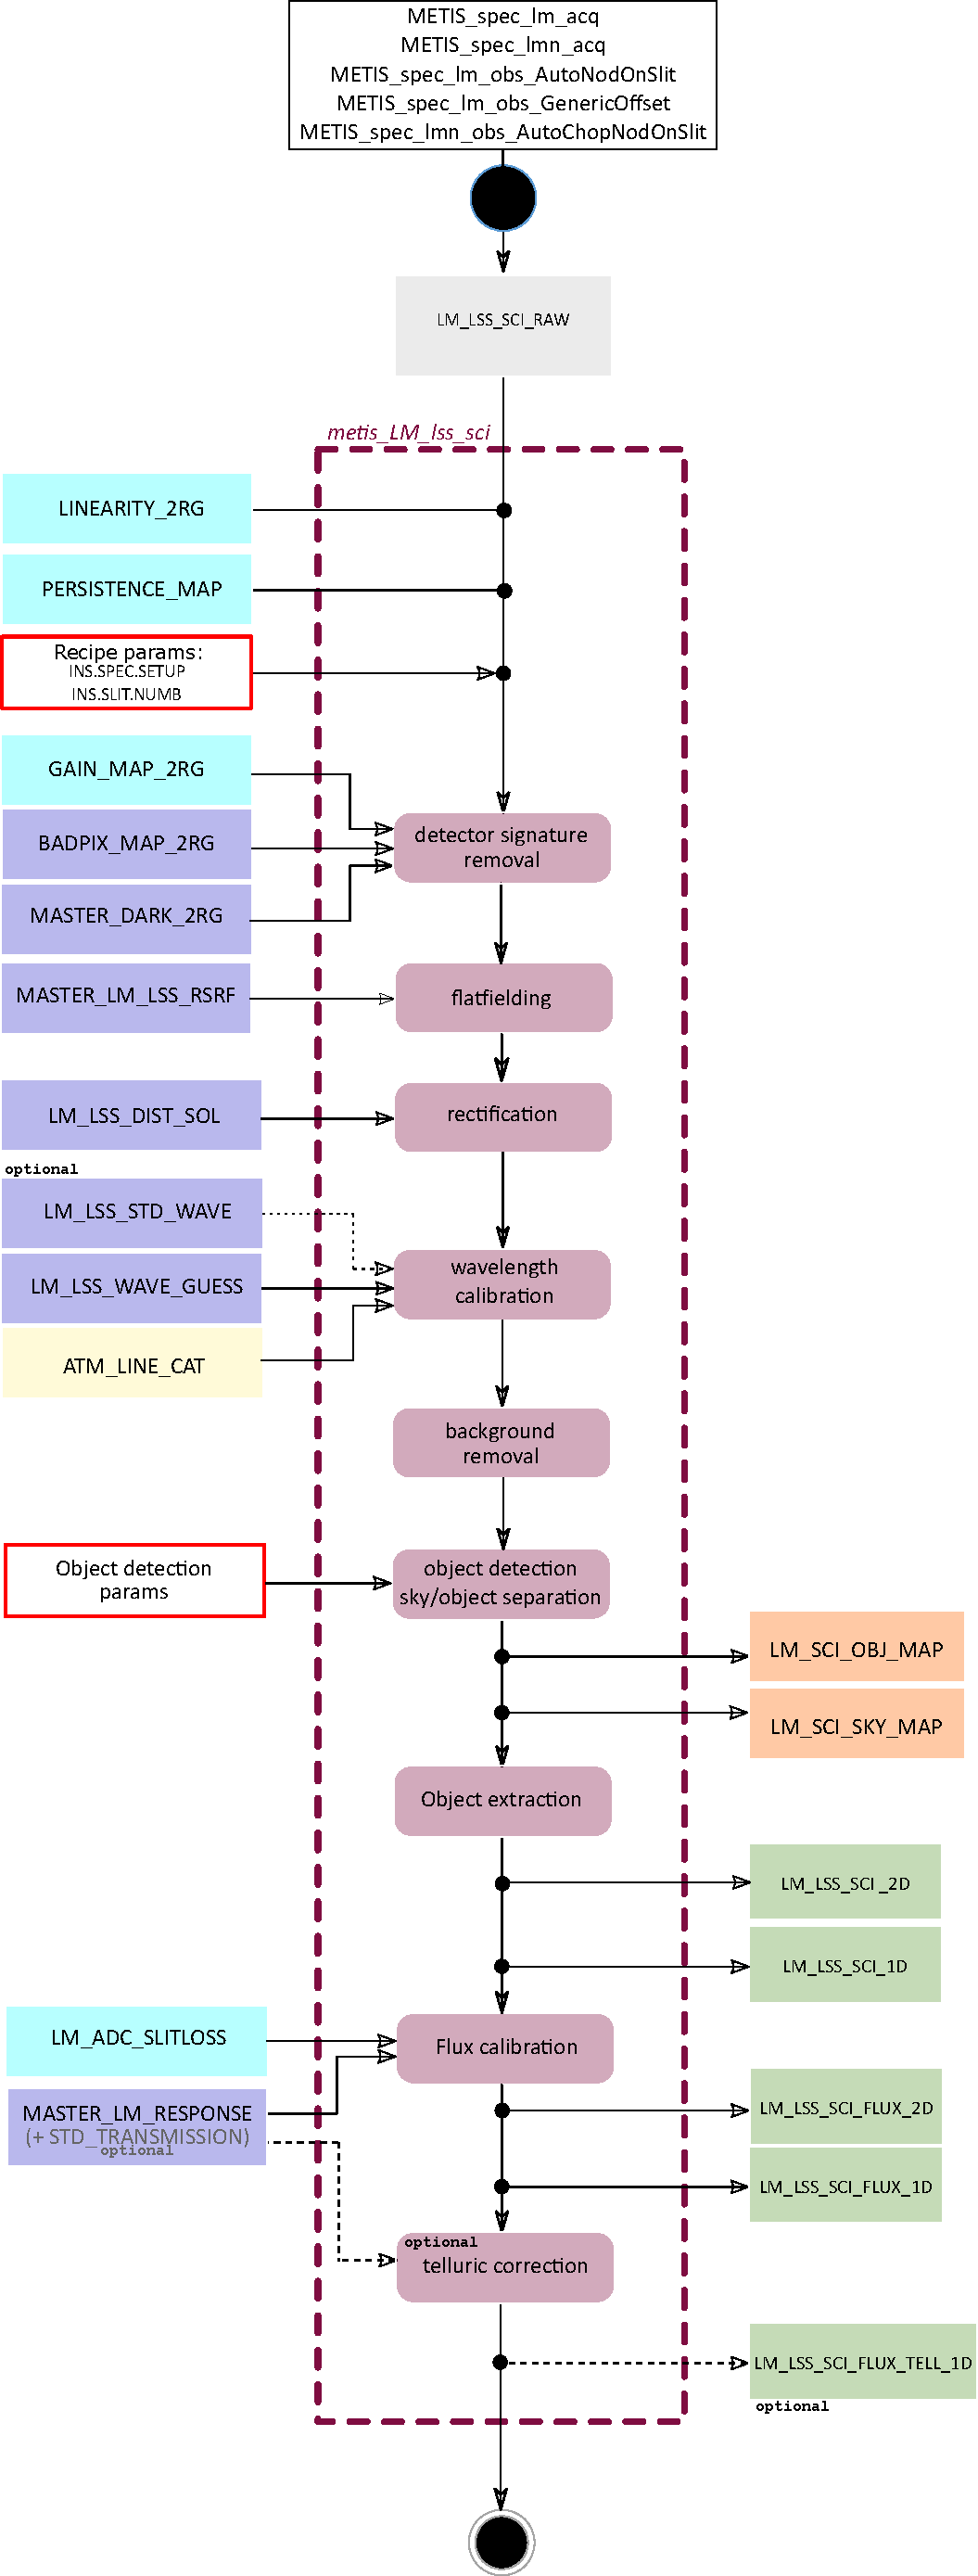
\includegraphics[width=0.36\textheight]{figures/metis_lm_lss_sci_v0.83.pdf}
    \notgenerated{flowchart: hand-drawn; the recipe declares no steps}
  \caption[Recipe: \REC*{metis_lm_lss_sci}]{\REC*{metis_lm_lss_sci} --
    Science reduction recipe.}
  \label{Fig:rec_lm_lss_sci}
\end{figure}
\clearpage

\begin{recipedef}
  Name:                & \REC{metis_lm_lss_sci} \\
  Purpose:             & Reduction of the LSS science star frames \\
%  Requirements:        & \REQ{METIS-XXXX} \\
%  Type:                & Calibration | Science | Technical \\
%  Templates:           & \TPL{...} \\
  Primary input:       & \RAW{LM_LSS_SCI_RAW} (N$\times$) \\
  Secondary inputs:    & \EXTCALIB{AO_PSF_MODEL} \\
                       & \PROD{BADPIX_MAP_2RG} (optional) \\
                       & \hyperref[dataitem:gain_map_det]{\STATCALIB*{GAIN_MAP_2RG}} \\
                       & \hyperref[dataitem:linearity_det]{\PROD*{LINEARITY_2RG}} \\
                       & \STATCALIB{LM_ADC_SLITLOSS} \\
                       & \PROD{LM_LSS_DIST_SOL} \\
                       & \PROD{LM_LSS_WAVE_GUESS} \\
                       & \PROD{MASTER_DARK_2RG} \\
                       & \PROD{MASTER_LM_LSS_RSRF} \\
                       & \PROD{MASTER_LM_RESPONSE} \\
                       & \EXTCALIB{PERSISTENCE_MAP} (optional) \\
                       & \PROD{STD_TRANSMISSION} (optional) \\
  Matched keywords:    & \FITS{DET.DIT} \\
                       & \FITS{DET.NDIT} \\
                       & \FITS{DRS.SLIT} \\
  Parameters:          & \CODE{metis_lm_lss_sci.parameter1}: string\newline Description of parameter 1 (\texttt{value2}, \underline{\texttt{value1}}) \\
  Algorithm:           & Fancy algorithm description follows ***TBD*** \\
  Output data:         & \PROD{LM_LSS_SCI_1D} \\
                       & \PROD{LM_LSS_SCI_2D} \\
                       & \PROD{LM_LSS_SCI_FLUX_1D} \\
                       & \PROD{LM_LSS_SCI_FLUX_2D} \\
                       & \PROD{LM_LSS_SCI_OBJ_MAP} \\
                       & \PROD{LM_LSS_SCI_SKY_MAP} \\
%  Expected accuracies: & \\
  QC1 parameters:      & \QC{QC LM LSS SCI FLUX NOISELEV} \\
                       & \QC{QC LM LSS SCI FLUX SNR} \\
                       & \QC{QC LM LSS SCI INTORDR LEVEL} \\
                       & \QC{QC LM LSS SCI NOISELEV} \\
                       & \QC{QC LM LSS SCI SNR} \\
                       & \QC{QC LM LSS SCI WAVECAL DEVMEAN} \\
                       & \QC{QC LM LSS SCI WAVECAL FWHM} \\
                       & \QC{QC LM LSS SCI WAVECAL NIDENT} \\
                       & \QC{QC LM LSS SCI WAVECAL NMATCH} \\
                       & \QC{QC LM LSS SCI WAVECAL POLYCOEFFn} \\
                       & \QC{QC LM LSS SCI WAVECAL POLYDEG} \\
\end{recipedef}


%------------------------------------------------------------------------------------------------------------------
\clearpage

\subsubsection{\REC*{metis_lm_lss_mf_model}:  Telluric correction}\label{rec:metis_lm_lss_mf_model}
The telluric correction will be done with the package \texttt{molecfit}\footnote{\url{https://www.eso.org/sci/software/pipelines/molecfit/molecfit-pipe-recipes.html}}\cite{molecfit}. It is based on the \texttt{telluricorr} package provided by \ac{ESO} and incorporates in three individual recipes, \REC{metis_lm_lss_mf_model}, which calculates the best-fit model, \REC{metis_lm_lss_mf_calctrans}, which creates a synthetic transmission curve, and \REC{metis_lm_lss_mf_correct}, which performs the actual telluric correction by means of the synthetic transmission.

\begin{figure}[ht]
  \centering
  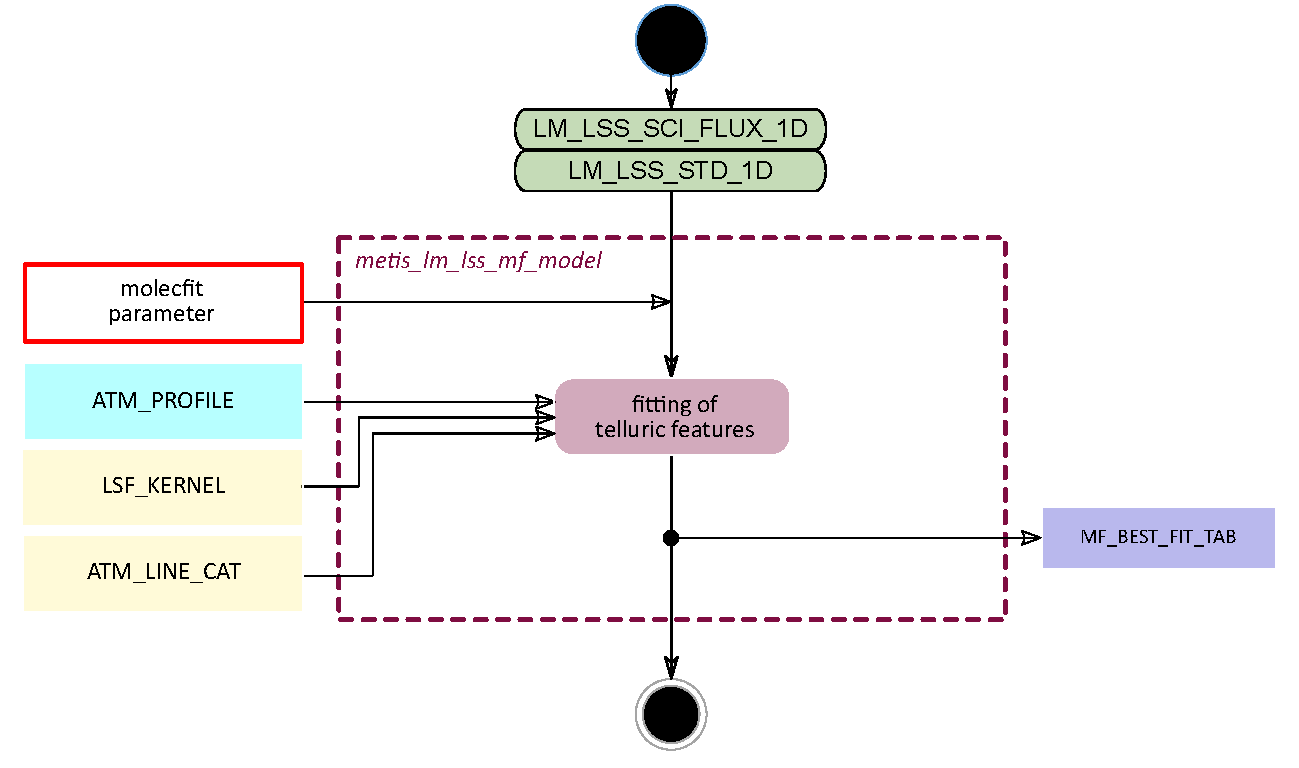
\includegraphics[width=0.5\textheight]{figures/metis_lm_lss_mf_model_v0.84.pdf}
    \notgenerated{flowchart: hand-drawn; the recipe declares no steps}
  \caption[Recipe: \REC*{metis_lm_lss_mf_model}]{\REC*{metis_lm_lss_mf_model} --
    Recipe to achieve the best-fit for the calculation of the synthetic transmission curve for the telluric correction.}
  \label{Fig:rec_lm_lss_mf_model}
\end{figure}
\clearpage

\begin{recipedef}
  Name:                & \REC{metis_lm_lss_mf_model} \\
  Purpose:             & Calculation of molecfit model \\
%  Requirements:        & \REQ{METIS-XXXX} \\
%  Type:                & Calibration | Science | Technical \\
%  Templates:           & \TPL{...} \\
  Primary input:       & \PROD{LM_LSS_SCI_FLUX_1D} \\
  Secondary inputs:    & \EXTCALIB{ATM_LINE_CAT} \\
                       & \EXTCALIB{ATM_PROFILE} \\
                       & \PROD{LM_LSS_SCI_1D} \\
                       & \STATCALIB{LSF_KERNEL} \\
  Matched keywords:    & \FITS{DRS.SLIT} \\
  Parameters:          & \CODE{metis_lm_lss_mf_model.parameter1}\newline Description of parameter 1 (\texttt{value2}, \texttt{value1}), default \texttt{value1} \\
  Algorithm:           & Fit of telluric features visible in the science input spectrum \\
                       & Determination of best-fit parameter set \\
  Output data:         & \PROD{MF_BEST_FIT_TAB} \\
%  Expected accuracies: & \\
  QC1 parameters:      & --- none --- \\
\end{recipedef}



%------------------------------------------------------------------------------------------------------------------
\clearpage
\subsubsection{\REC*{metis_lm_lss_mf_calctrans}:  Telluric correction}\label{rec:metis_lm_lss_mf_calctrans}

\begin{figure}[ht]
  \centering
  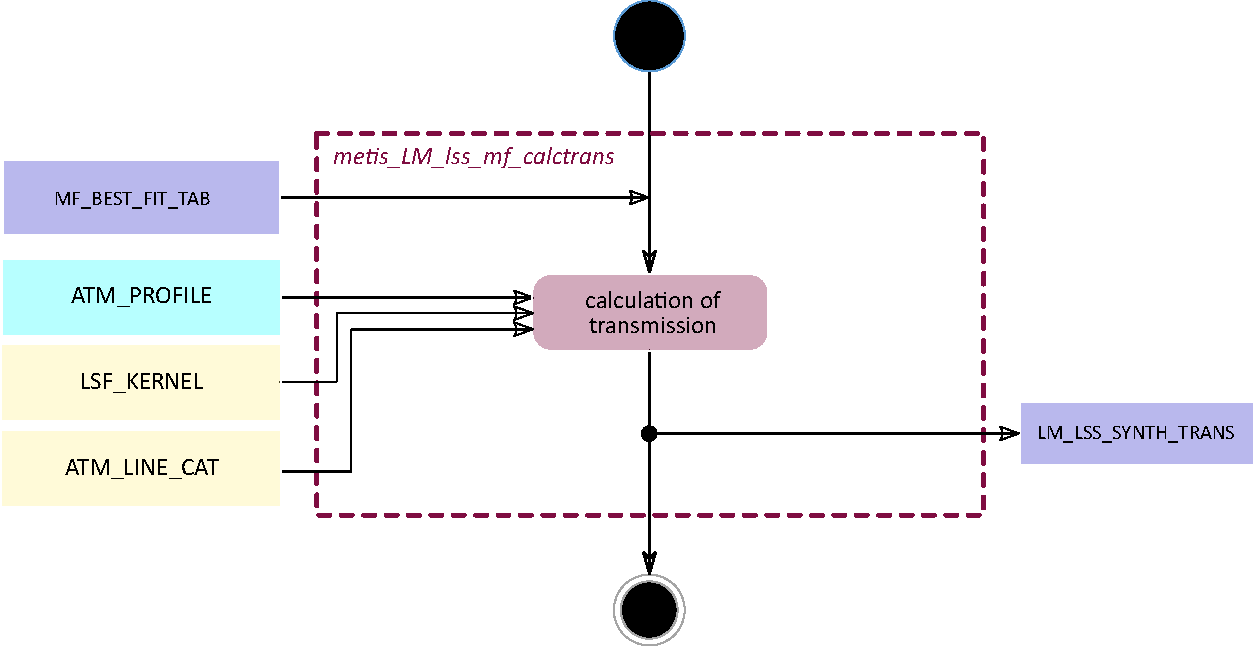
\includegraphics[width=0.5\textheight]{figures/metis_lm_lss_mf_calctrans_v0.83.pdf}
    \notgenerated{flowchart: hand-drawn; the recipe declares no steps}
  \caption[Recipe: \REC*{metis_lm_lss_mf_calctrans}]{\REC*{metis_lm_lss_mf_calctrans} --
    Recipe to calculate the synthetic transmission to be applied as telluric correction.}
  \label{Fig:rec_lm_lss_mf_calctrans}
\end{figure}
\clearpage

\begin{recipedef}
  Name:                & \REC{metis_lm_lss_mf_calctrans} \\
  Purpose:             & Calculation of transmission function \\
%  Requirements:        & \REQ{METIS-XXXX} \\
%  Type:                & Calibration | Science | Technical \\
%  Templates:           & \TPL{...} \\
  Primary input:       & \PROD{MF_BEST_FIT_TAB} \\
  Secondary inputs:    & \EXTCALIB{ATM_LINE_CAT} \\
                       & \EXTCALIB{ATM_PROFILE} \\
                       & \STATCALIB{LSF_KERNEL} \\
  Matched keywords:    & \FITS{DRS.SLIT} \\
  Parameters:          & \CODE{metis_lm_lss_mf_calctrans.parameter1}: string\newline Description of parameter 1 (\texttt{value2}, \underline{\texttt{value1}}) \\
  Algorithm:           & Fancy algorithm description follows ***TBD*** \\
  Output data:         & \PROD{LM_LSS_SYNTH_TRANS} \\
%  Expected accuracies: & \\
  QC1 parameters:      & --- none --- \\
\end{recipedef}



\subsubsection{\REC*{metis_lm_lss_mf_correct}:  Telluric correction}\label{rec:metis_lm_lss_mf_correct}

\begin{figure}[ht]
  \centering
  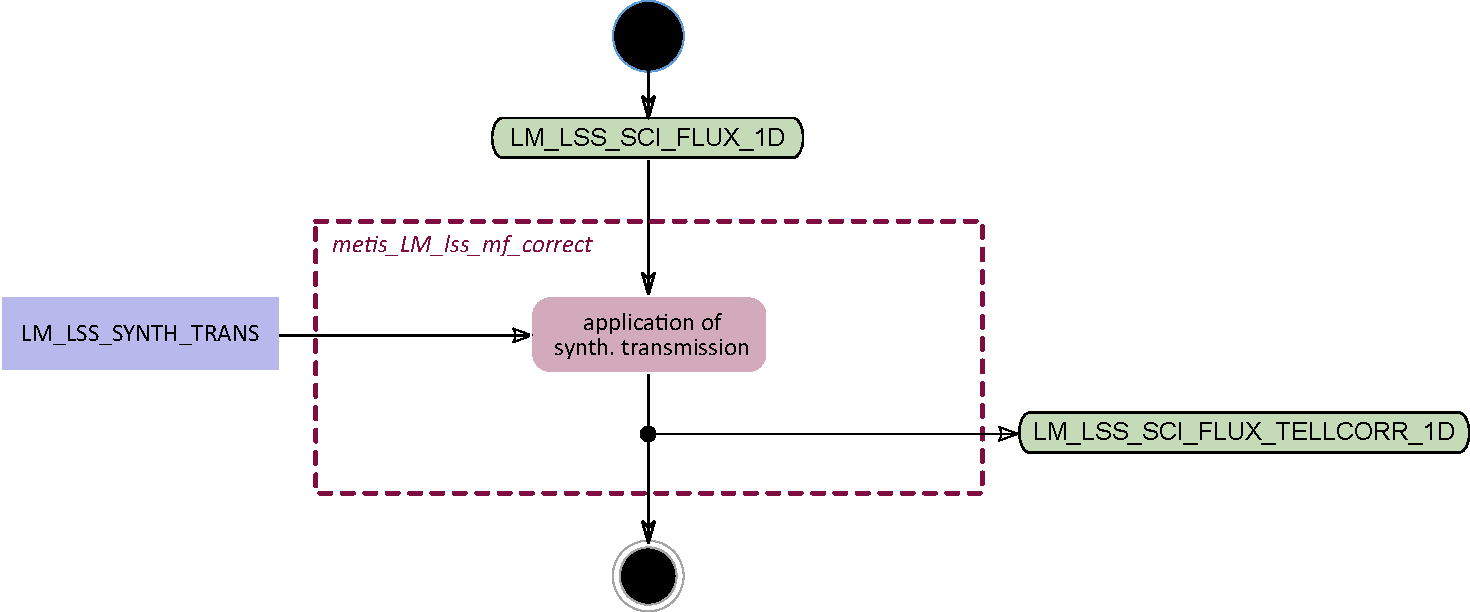
\includegraphics[width=0.5\textheight]{figures/metis_lm_lss_mf_correct_v0.83.pdf}
    \notgenerated{flowchart: hand-drawn; the recipe declares no steps}
  \caption[Recipe: \REC*{metis_lm_lss_mf_correct}]{\REC*{metis_lm_lss_mf_correct} --
    Recipe to apply the telluric correction.}
  \label{Fig:rec_lm_lss_mf_correct}
\end{figure}
\clearpage

\begin{recipedef}
  Name:                & \REC{metis_lm_lss_mf_correct} \\
  Purpose:             & Application of the telluric correction \\
%  Requirements:        & \REQ{METIS-XXXX} \\
%  Type:                & Calibration | Science | Technical \\
%  Templates:           & \TPL{...} \\
  Primary input:       & \PROD{LM_LSS_SCI_FLUX_1D} \\
  Secondary inputs:    & \PROD{LM_LSS_SYNTH_TRANS} \\
  Matched keywords:    & \FITS{DRS.SLIT} \\
  Parameters:          & \CODE{metis_lm_lss_mf_correct.parameter1}\newline Description of parameter 1 (\texttt{value2}, \texttt{value1}), default \texttt{value1} \\
  Algorithm:           & Apply telluric correction, i.e. divide the input science spectrum by the synthetic transmission. \\
  Output data:         & \PROD{LM_LSS_SCI_FLUX_TELLCORR_1D} \\
%  Expected accuracies: & \\
  QC1 parameters:      & --- none --- \\
\end{recipedef}





